\documentclass[12pt, a4paper]{scrartcl}
\usepackage[utf8]{inputenc}
\usepackage{graphicx}
\usepackage{amsmath, amsthm, amssymb, textcomp}
\usepackage{setspace}
\usepackage{paralist}
\usepackage{graphicx}
\usepackage{caption}
\graphicspath{{WSK_im/}} %Graphic is in a folder named WSK_im in the currend directory
\usepackage{float}
\usepackage{authblk}
\renewcommand\Authfont{\fontsize{12}{14.4}\selectfont}
\title{Bayesian probability theory - Lesson 4}

\author{Wolfgang von der Linden}
\date{Transscript}

\begin{document}
\setlength{\parindent}{0pt}
\maketitle
\onehalfspacing

Welcome to the forth unit of the course on Bayesian probability theory. 
My name is Wolfgang von der Linden and I will enable you to help Captain Bayes and her crew to solve their new tasks.
This unit is dedicated to \textbf{combinatorics} or "the art of counting".
We will count the possibilities to \textit{arrange different objects}, we will determine the probability for \textit{drawing objects} in different settings and discuss different strategies to \textit{distribute objects} into boxes.
Before we begin to derive combinatorial solutions to the problems posed, here is a brief justification as to why counting is important.
We have already seen that probabilities in many cases have to do with counting various types of outcomes. This is of crucial importance for instance for example in statistical physics, therefore proper counting is crucial.\\

\section*{Arranging distinguishable objects}
In the adventure, Pascal thought about the number of different arrangements of jars, each of which has different colors. 
As Captain Bayes conjectured, the number of arrangements or \textbf{permutations} can be derived as follows:
For the first object to be placed on the first position of the shelf, we have N choices,  for the second we have N-1 choices and so on, resulting in N times N-1 times  N-2 times all way down to times 1.
This function is very important and is called \textbf{factorial} and denoted by an exclamation mark $N!$.
%4_1
 \begin{figure}[H]
	\centering
	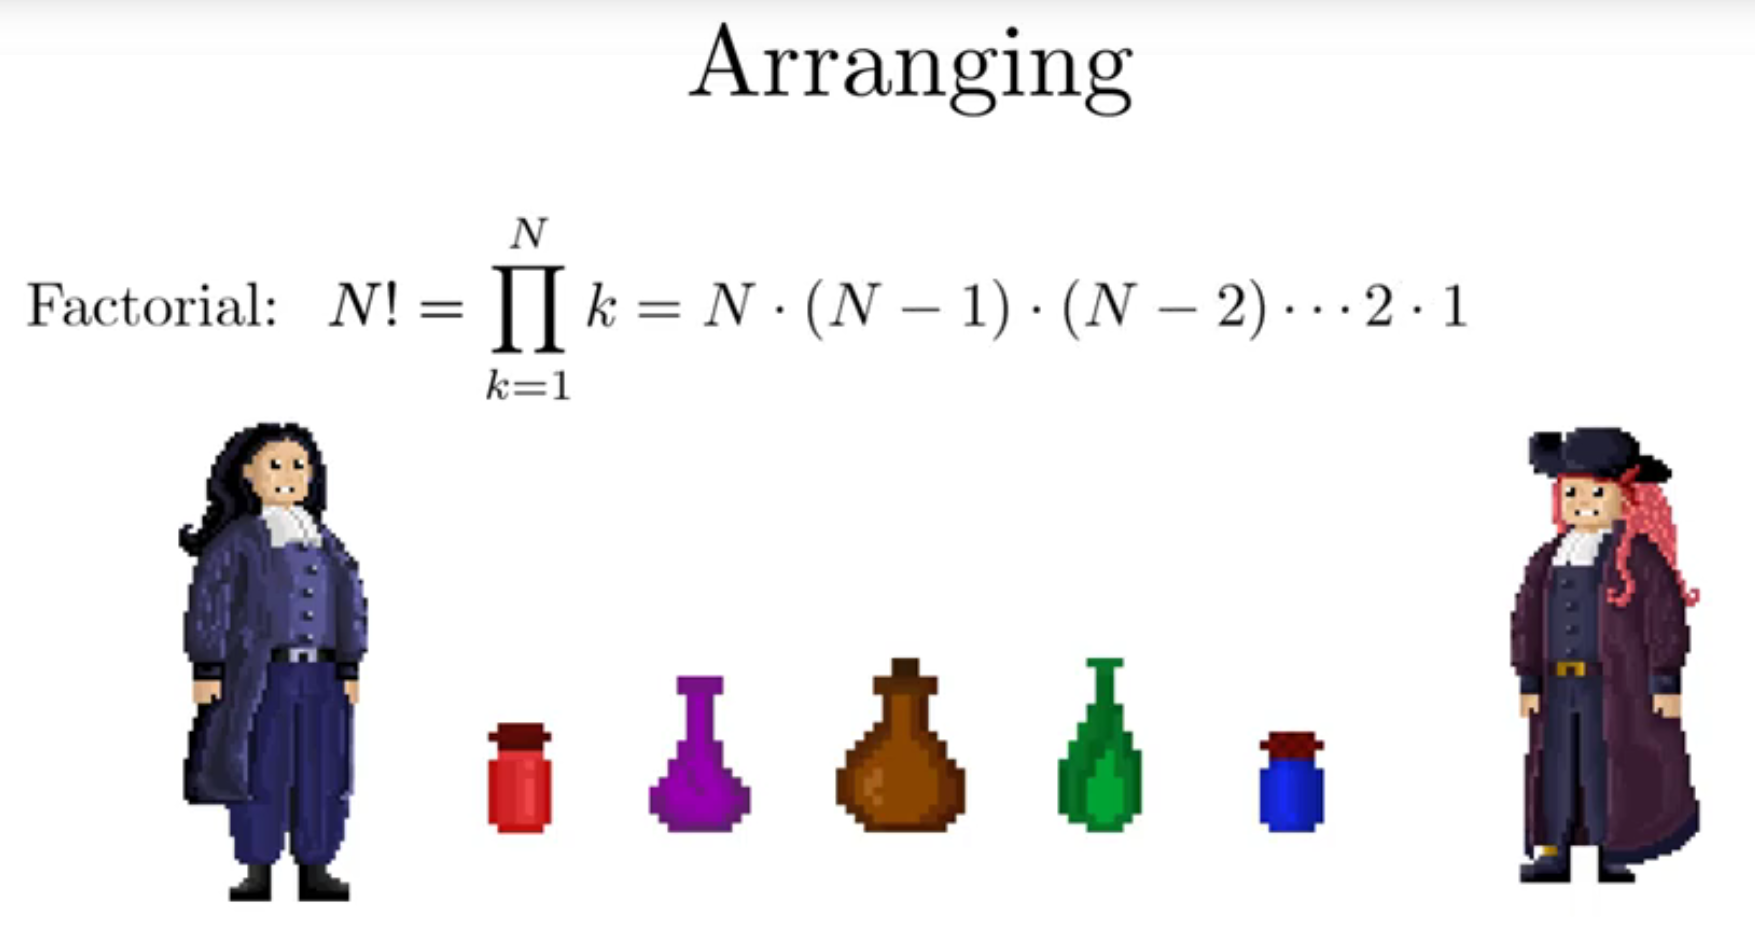
\includegraphics[width=0.75\textwidth]{4_1.png}
\end{figure}
\fbox{\parbox{\linewidth}{\textbf{Question 1.} What is the factorial of 4?\\
4!=.......
}}\\
In the example of 5 coloured bottles the number of permutations is $5!=120$\\
\fbox{\parbox{\linewidth}{\textbf{Question 2.} What is the factorial of 10?\\
10!=.......
}}\\

We see the factorial rapidly increases with N. (For example 100! is an integer with 155 digits.) 
Since the factorial function is defined recursively, it is hard to evaluate. The so-called \textbf{Stirling formula} - though first introduced by \textbf{Moivre} - provides an approximation which is especially useful for \textit{large factorials}.
\begin{equation*}\boxed{N! \approx \sqrt{2\pi N}\left( \frac{N}{e}\right)^N
}\end{equation*}\\
\begin{equation*}\boxed{\sqrt{2\pi}N^{N+1/2}exp(-N)\leq N!\leq N^{N+1/2}exp(-N+1)
}\end{equation*}\\
One usually uses the logarithm version of the Stirling formula which simplifies analytic calculations a lot.\\

\begin{equation*}\boxed{ln(N!)\approx N ln(N)-N+\frac{ln(2\pi N)}{2}
}\end{equation*}\\
\begin{equation*}\boxed{\left(N+\frac 12 \right)ln(N)-N-\frac 12 ln\left(\frac{\pi}{2}\right)\leq ln(N!)\leq\left(N+\frac 12\right)ln(N) - N+1
}\end{equation*}\\
\fbox{\parbox{\linewidth}{\textbf{Question 3.} Which of the following stements/estimations are true?\\
a) The factorial function increases faster than polynomial functions.\\
b) A rough approximation for the factorial is given by $N!\approx Nlog(N)$.\\
c) A rough approximation for the factorial is given by $N! \approx \sqrt{2\pi N}\left( \frac{N}{e}\right)^N$.\\
d) The factorial function increases faster than exponential functions.
}}\\
\section*{Arranging groups of indistinguishable objects}
Captain  Bayes was wondering how the number of arrangements changes if one adds additional copies of jars with the very same color.
The difference to the previous problem is that now some jars are \textbf{indistinguishable} and \textit{exchanging them results in the same arrangement}.
Let’s first consider objects with two colors only. So for example some of them ($K_1$) having red color and others ($K_2$) are brown.

Now the total number of permutations of all objects - which we have derived before - must be divided by those permutations which lead to exactly the same arrangement - which means we have to \textit{divide by the possible permutations of the objects with the same color}.
%4_2
 \begin{figure}[H]
	\centering
	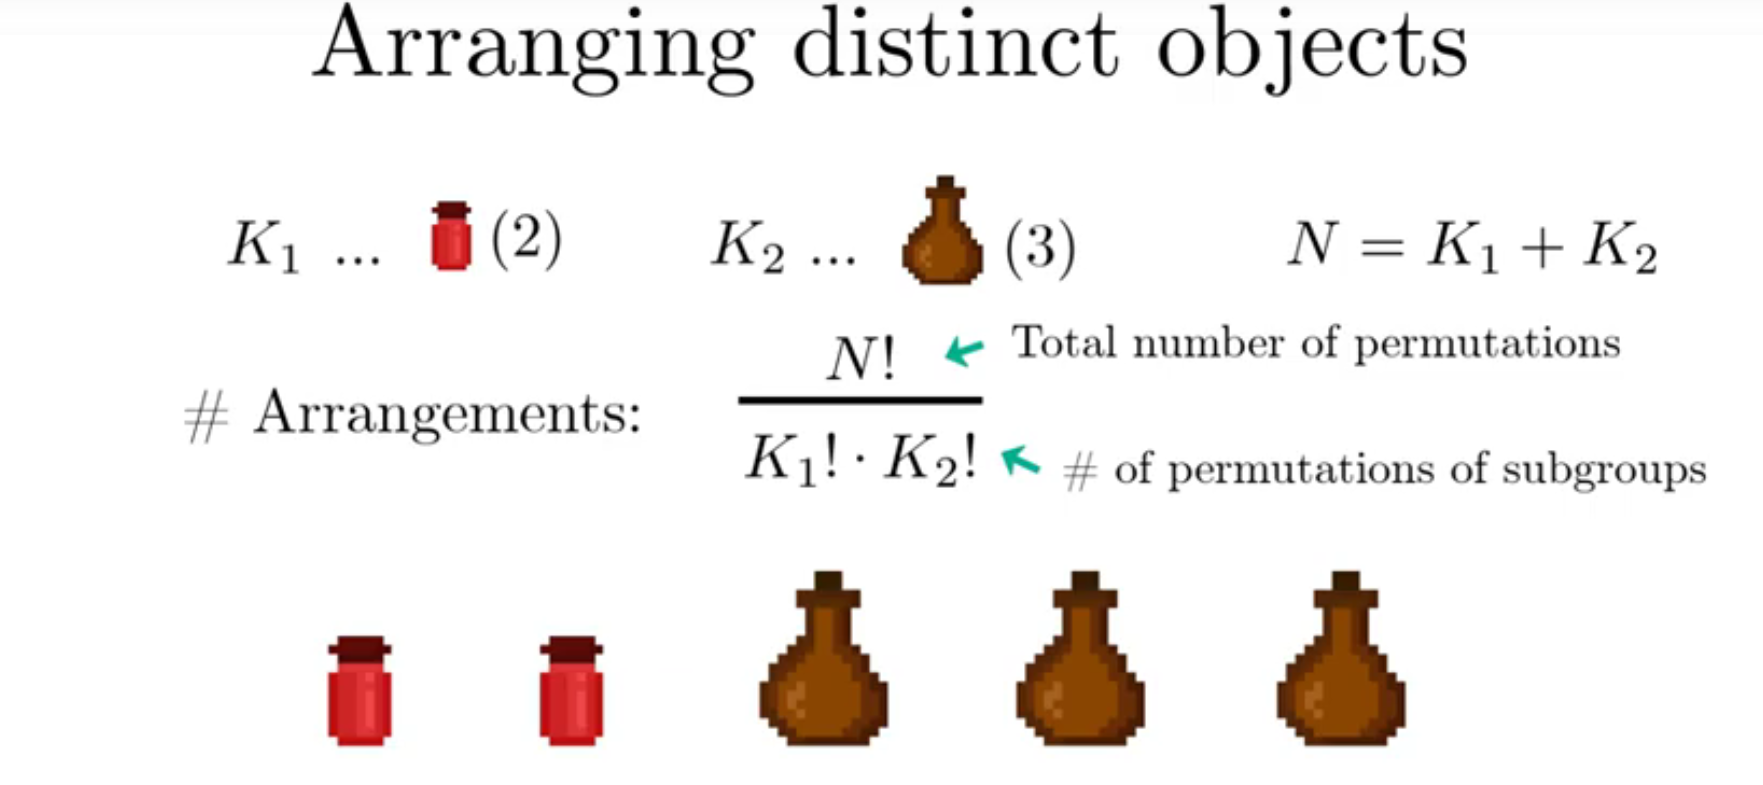
\includegraphics[width=0.75\textwidth]{4_2.png}
\end{figure}
This term is called the \textbf{binomial coefficient}. 
We say \textit{``N choose K''} ${N\choose K}$ for the number of possibilities to choose K out of N elements. In our example of arranging choosing corresponds to choosing the positions for the brown bottles. The number of possibilities to arrange three brown bottles and two red jars is thus given by ${5 \choose 3}$ = 10.\\


In this context, the \textbf{binomial theorem} for two real numbers a and b is also worth mentioning.
\begin{equation*}\boxed{(a+b)^N = \sum_{K=0}^{N}{N\choose K}a^Nb^{N-K}
}\end{equation*}\\
\fbox{\parbox{\linewidth}{\textbf{Question 4.} Which of the following stements are true?\\
a) ${6 \choose 4}={6\choose 2}$\\
b) The coefficient of $x^3y^{17}$ in $(x+y)^{20}$ is given by ${20\choose 3}$.\\
c) ${8\choose 3} = \frac{8^3}{3!5!}$
}}\\

\subsection*{Pascal’s triangle }
As already mentioned in the episode, Pascal developed a nice way to derive these binomial coefficients using a triangle.
The recipe is as follows:\\
      Start with a  triangle of three ``1''.\\
      Now add two neighboring numbers of the row and write the result below the center of these two numbers\\
      Close the row on the left and right edge with a ``1''.\\
Now repeat steps 2 and 3.\\
That way we produce a triangle that contains the binomial coefficients: The N-th row contains the binomial coefficients ${N \choose k} $\\
%4_3
 \begin{figure}[H]
	\centering
	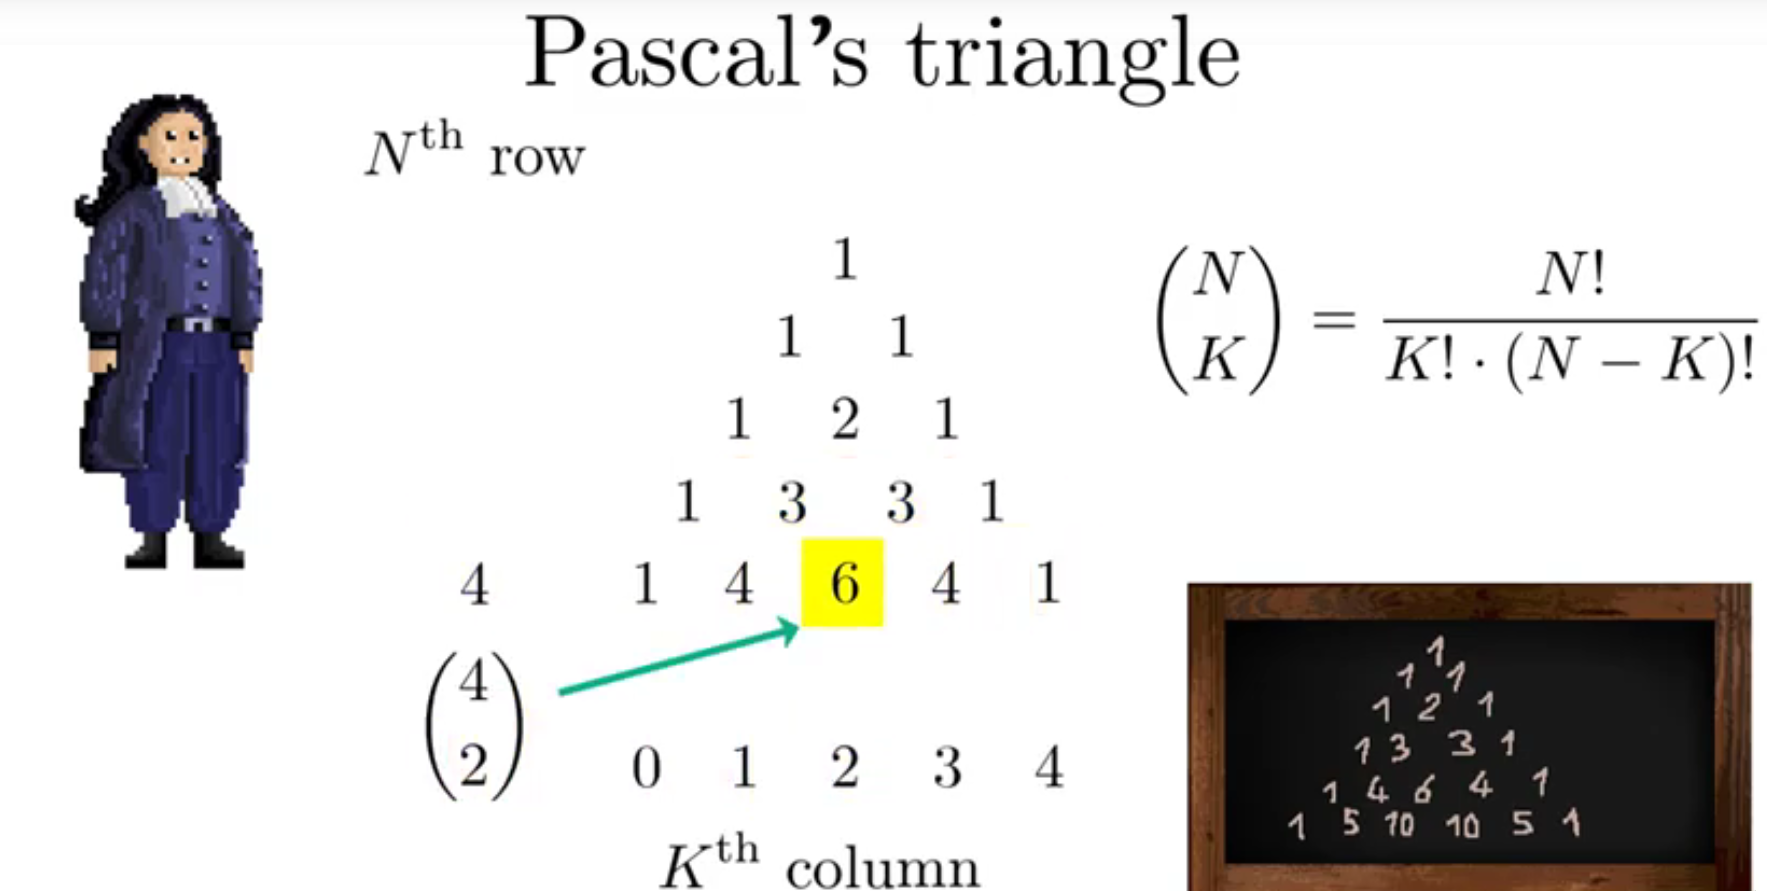
\includegraphics[width=0.75\textwidth]{4_3.png}
\end{figure}
\fbox{\parbox{\linewidth}{\textbf{Question 5.} Which relations are correct?\\
a) ${N+1\choose K} = {N\choose K}+{N\choose K-1}$\\
b) ${N+1\choose K+^1} = {N\choose K}+{N\choose K+1}$\\
c) ${N\choose K} = {N\choose N-K}$\\
d) ${N+1\choose K} = {N\choose K}+{N\choose K+1}$
}}\\

The question of arranging objects that can be divided into subsets according to their color can easily be generalised to more than two colors. We assume $K_1, K_2, K_3$, and so on elements in the subsets with a total of N elements.
Then N! is the total number of permutations and $K_i!$ the number of permutations for the elements of subset i.
So the number of combinations or arrangements is given by the following term which is called \textbf{Multinomial coefficient}.\\
\begin{equation*}\boxed{{N\choose \{K_i\}}=\frac{N!}{\Pi_{i=1}^LK_i!}
}\end{equation*}\\

Let’s illustrate that with the number of words - let's leave aside their meaning - you can form with the letters a, b, and c, if you use 3 a 4 b and 5 c
The number of words is surprisingly large.\\
%4_4
 \begin{figure}[H]
	\centering
	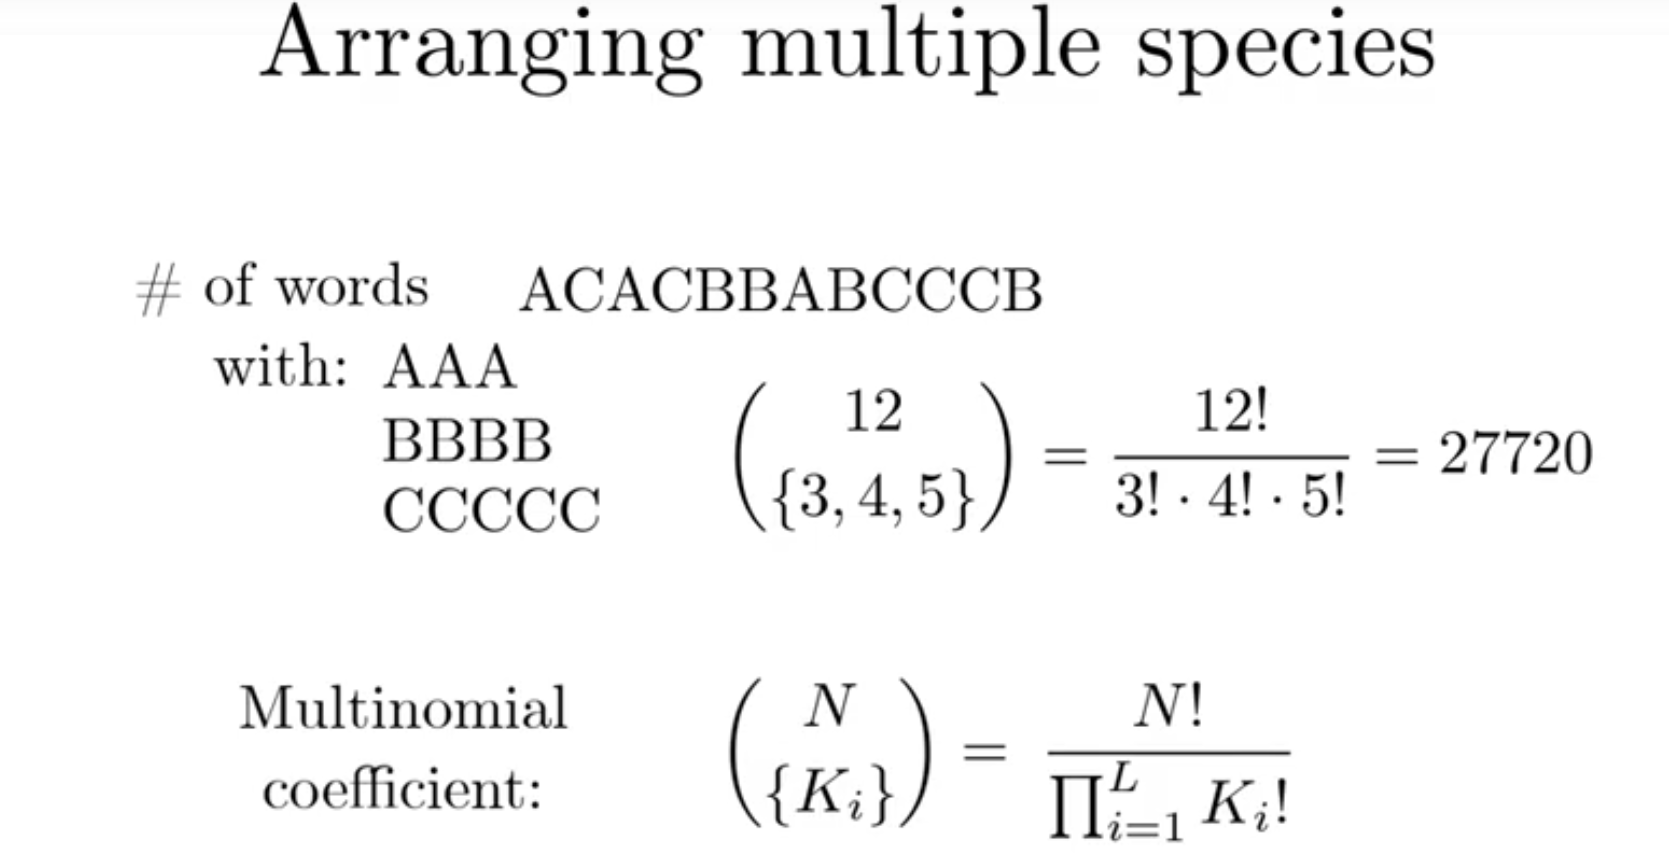
\includegraphics[width=0.75\textwidth]{4_4.png}
\end{figure}

\section*{Drawing objects with replacement}
Now, let’s assist Bernoulli with his task, to compute the probability to draw 5 apricots and 3 plums out of a pot, where the probability for an apricot is one third in a single draw.
Bernoulli does \textit{not care about the order} the dried fruits are drawn from the clay pot. Only the \textit{total numbers of apricots and plums} is important. There are several elementary events that lead to the desired amount of ingredients.
Since theses events are \textit{exclusive} we can apply the simplified sum rule.
Recall that Bernoulli made sure that the condition for drawing the second fruit was the same as that for the first, by putting the drawn fruit back into the clay pot. 
Therefore the individual draws are \textit{uncorrelated} and according to the previous unit, the simplified product rule applies\\
%4_5
 \begin{figure}[H]
	\centering
	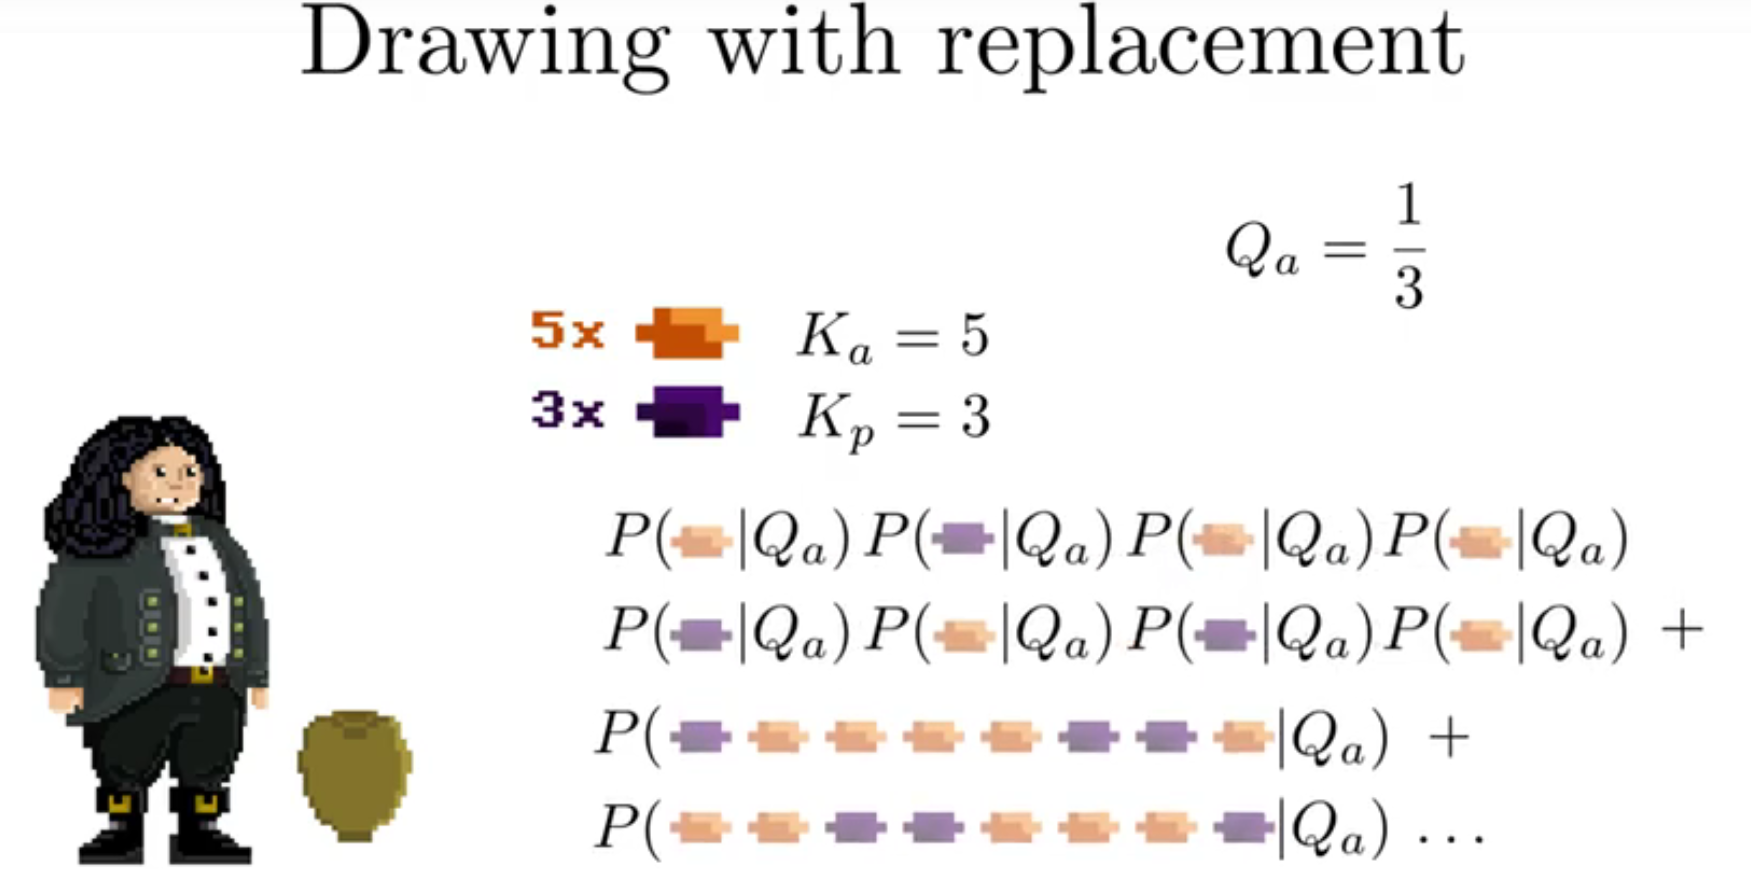
\includegraphics[width=0.75\textwidth]{4_5.png}
\end{figure}
\textit{Note that for the logical AND the order is irrelevant, which is also the case for the independent draws.}
\begin{equation*}\boxed{P(K_a=5,K_p=3|Q_a)=XQ_a^5(1-Q_a)^3
}\end{equation*}\\
The remaining task is simply to determine the number of arrangements X in which the dried fruits can be drawn. But this is the same as the number of arrangements of jars of two different colors that we have previously shown to be the binomial coefficient $X={8 \choose 3}$.
For the numerical result we evaluate ${8 \choose 3}$ which is 56 and obtain a probability of 6.8\%.
The experiment just discussed is called a \textbf{Bernoulli experiment}, which has \textit{2 outcomes}, one with probability Q and the complementary one with 1-Q.
The probability to obtain K times the first outcome in N attempts is given by the binomial distribution we mentioned in the last lesson.\\
\begin{equation*}\boxed{P_B(K|N,Q)={N\choose K}Q^K(1-Q)^{N-K}
}\end{equation*}\\
\fbox{\parbox{\linewidth}{\textbf{Question 6.} What is the probability to have 5 times heads when tossing a fair coin 7 times?\\
a) P(5 heads$|$N=7)$\approx$17\%\\
b) P(5 heads$|$N=7)=${7 \choose 2}2^{-7}$\\
c) P(5 heads$|$N=7)${5\choose 2}0.5^5(1-0.5)$
}}\\

The generalization from two to L colors that can be drawn from the pot is straight forward.
The probability for obtaining the color i with a frequency of $K_i$ in a total number of draws N is given by the multinomial distribution
\begin{equation*}\boxed{P_M(K_1,K_2,...|Q_1,Q_2,...)=\frac{N!}{\prod_iK_i!}\prod_iQ_i^{K_i}}\end{equation*}\\
The term $Q_i$ describes the probability for drawing color i in a single draw, so in our example this is the \textbf{relative frequency} of the individual colors.
Interestingly, for the fluctuations there is a negative correlation since the total number N is fixed.
%4_6
 \begin{figure}[H]
	\centering
	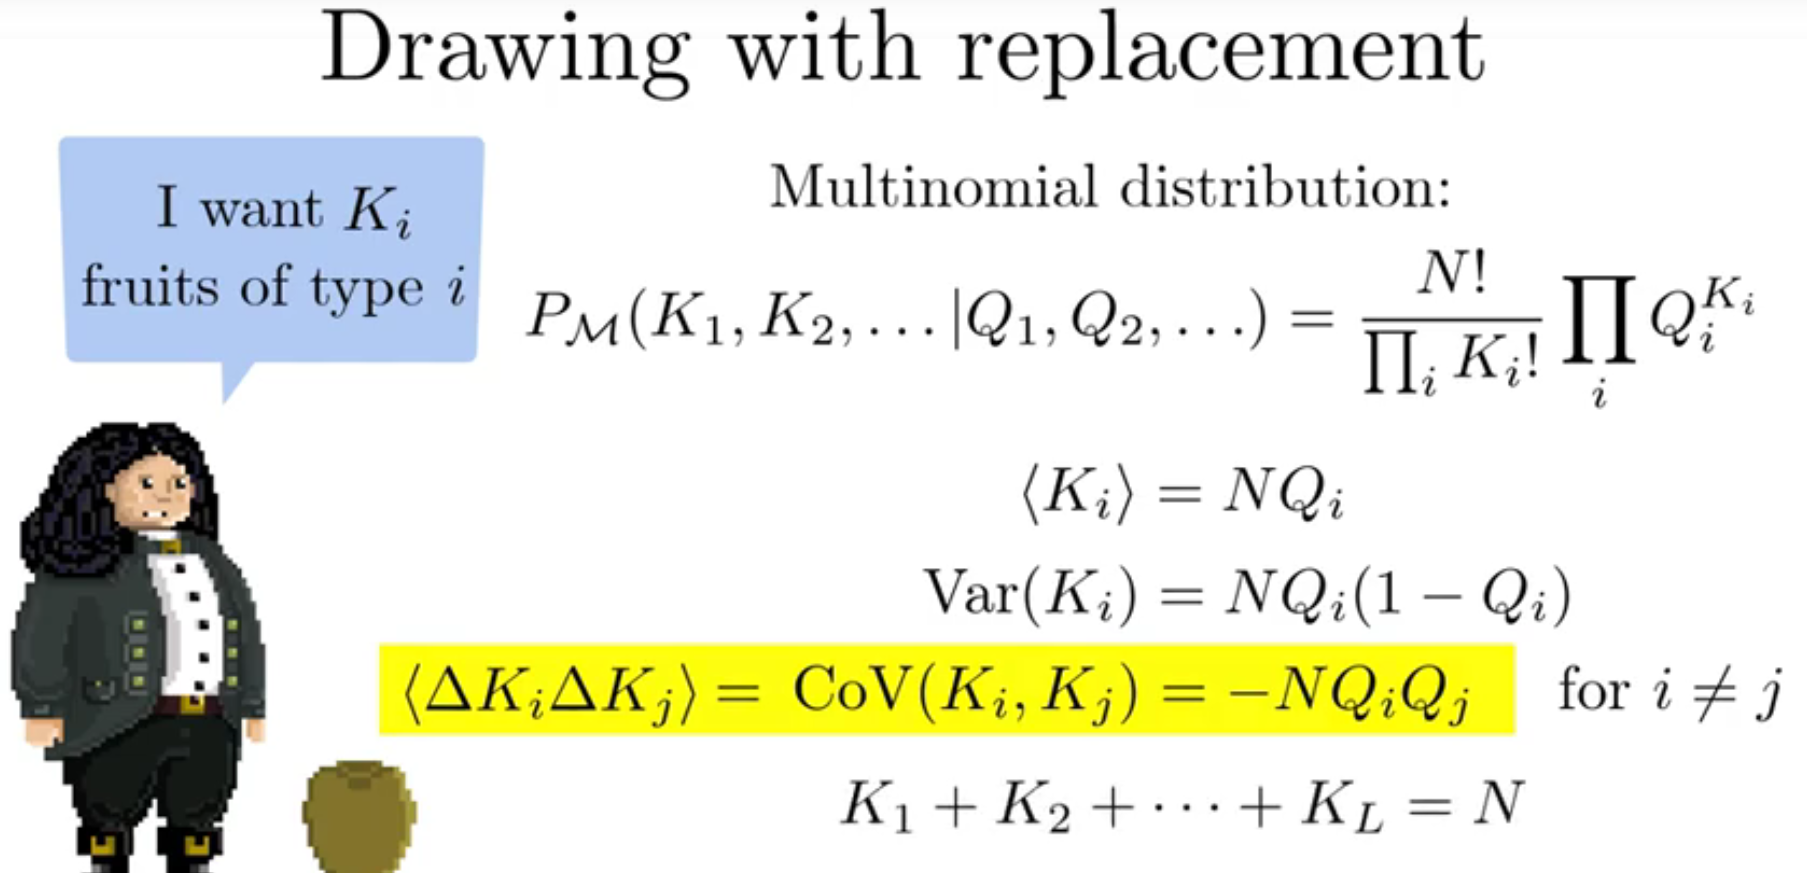
\includegraphics[width=0.75\textwidth]{4_6.png}
\end{figure}
We can also readily generalize the binomial theorem to the multinomial theorem.\\%%
\begin{equation*}\boxed{(a_1+a_2+..+a_L)^N=\sum_{\{K_i\}, K1+..+K_l=N}{N\choose{K_i}}\prod_{i=1}^{L}a_i^{K_i}
}\end{equation*}\\
\fbox{\parbox{\linewidth}{\textbf{Question 8.} What is the probability to have 3 times a six and 4 times a one when throwing a dice 8 times?\\
a) 0.07\%\\
b) 2\%\\
c) ${8 \choose \{4,1,3\}}\frac{1}{6^7}\frac{4}{6}$\\
d) ${7 \choose 4}\frac{1}{6^7}$
}}\\
\section*{Drawing objects without replacement}
Now we follow Captain Bayes' recommendation not to put the fruits back into the pot, i.e. \textbf{without replacement}.\\
The general situation is the following. Originally there are $N_a$ apricots and $N_p$ plums, so in total N fruits in the clay pot. We draw at random K elements.
What is the probability that we find $K_a$ apricots and $K_p$ plums?\\
We use the classical definition of probability as the \textit{ratio of the number of favorable outcomes divided by the total number of outcomes}. 
An \textbf{outcome} in this case is a \textit{sequence of elements of apricots and plums of length K}.
The total number of different outcomes is given by ${N \choose K}$ which is the number of subsets of size K we can form. 
Similarly, ${N_a \choose K_a}$ is the number of subsets we can form if we only consider apricots.
Likewise, we obtain the number of subsets we can form if we only consider plums.
So the product gives the number of favorable outcomes and for the desired probability we mearly have to \textit{divide by the total number of outcomes}.
Finally, when K is the number of fruits drawn from the pot with $N_a$ apricots of N fruits in total, the probability to find $K_a$ apricots is described by the \textbf{hypergeometric distribution}.\\%
\begin{equation*}\boxed{P_H(K_a|K,N,N_a)=\frac{{N_a\choose K_a}{N-N_a\choose K-K_a}}{{N\choose K}}
}\end{equation*}\\


For the problem considered by Bernoulli, we have just deduced that we need the total number of fruits in the pot, which is given by Ernesto at the end of the last episode as 30 fruits.
With 10 apricots and 20 plums in total we can now evaluate the probability to obtain 5 apricots and 3 plums when drawing without replacement.
Before evaluating this probability we will exercise our ability to estimate! What do you think, will the probability be higher or lower than the 6.8\% we got when drawing with replacement?\\

\fbox{\parbox{\linewidth}{\textbf{Question 9.}What do you think? How will the probabilitiy to draw 5 apricots and 3 plums out of a clay pot with a ratio of 1:2 change, when switching from "drawing with replacement" to "drawing without replacement"?\\
a) P will increase\\
b) P will decrease\\
}}\\

(The probability is approximately 5\%, so lower.)
The reason is that the ratio we would like to draw (5 to 3) is kind of opposite to the ratio of fruits inside (1 to 2). If there were 20 apricots and 10 plums in the pot, the probability when drawing without replacement would be greater than that with replacement.
%4_7
 \begin{figure}[H]
	\centering
	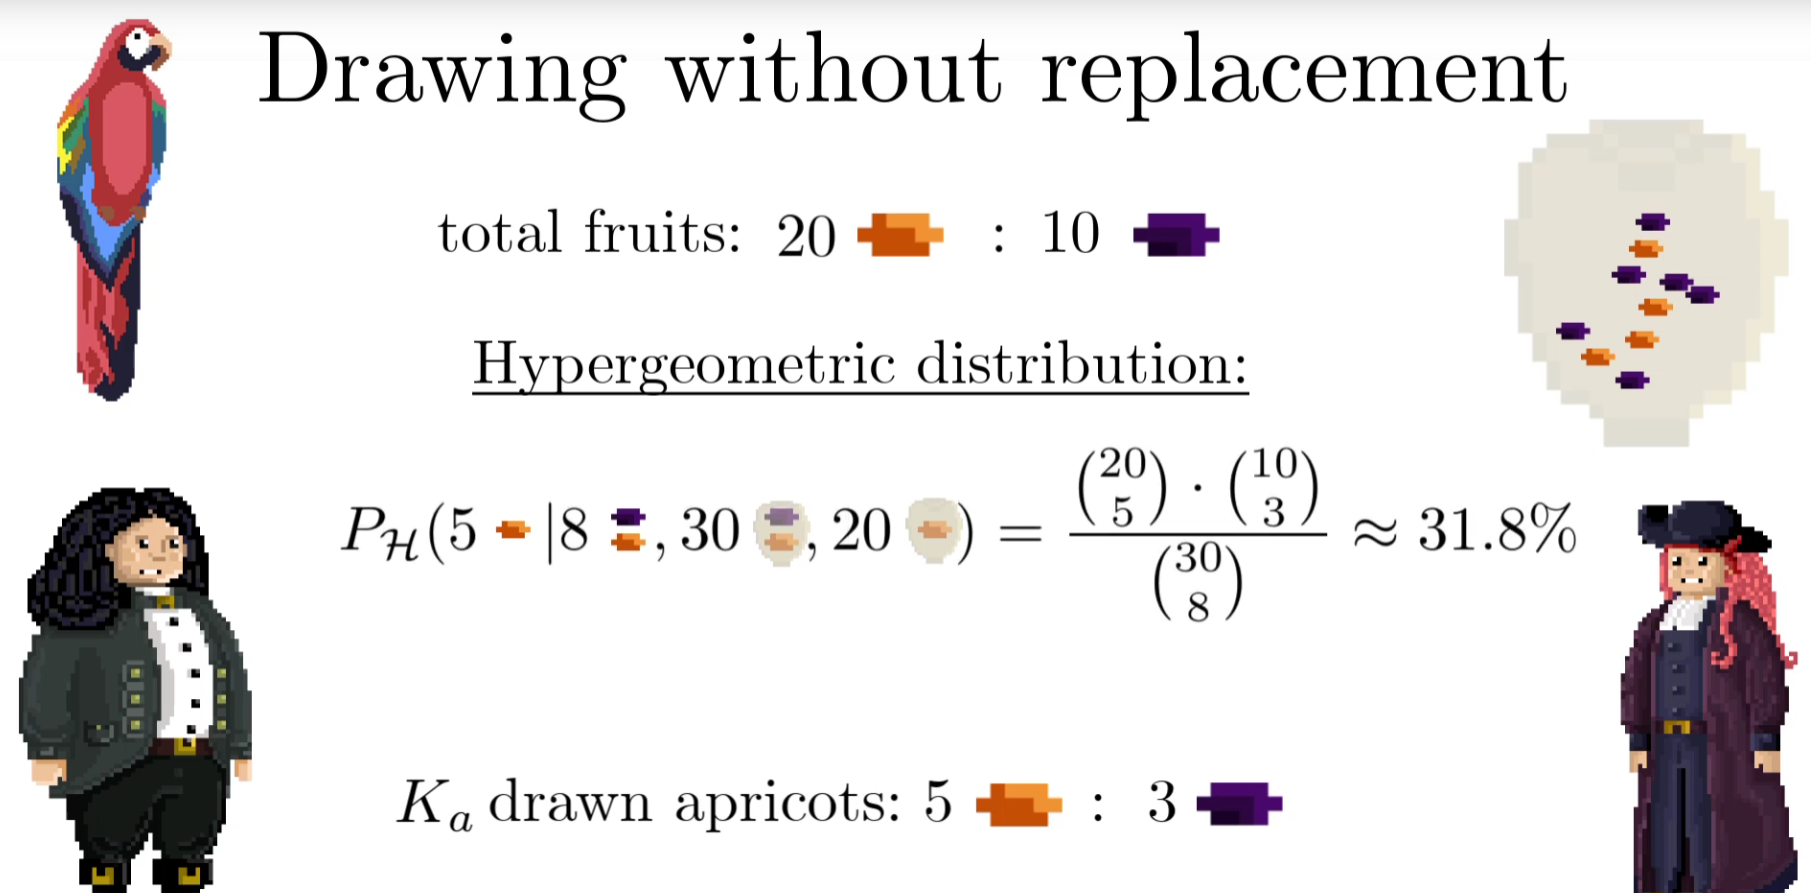
\includegraphics[width=0.75\textwidth]{4_7.png}
\end{figure}
A second estimation question: How will the probability change if there were 10 times as many fruits inside the pot?\\

\fbox{\parbox{\linewidth}{\textbf{Question 10.}How will the probability change when increasing the numbers of fruits in the pot by a factor of 10, when we're still drawing 5 apricots and 3 plums without replacement?\\
a) P will decrease further\\
b) P will increase and be comparable to drawing with replacement
}}\\

The result is 6.7\% and it strongly resembles the result obtained when drawing with replacement. The reason is, that removing fruits now hardly changes the odds. 
(You will have ample opportunity to compare the results in the pluto notebook.)\\

The hypergeometric distribution is of importance in \textit{mark-recapture techniques} for population estimation, which is used in ecology to estimate population sizes of animals or in epidemiology to track the spread of diseases. 
For concreteness, let us consider the following example. Assume that the total number of fish in a lake is N. Out of these $N_1$ fish are caught, tagged with a red dot and released. After a sufficiently long period of time to allow for mixing K fish are caught.
What is the probability for having $K_1$ labeled fish in the sample if N is known? This probability is given by the hypergeometric distribution
%4_8
 \begin{figure}[H]
	\centering
	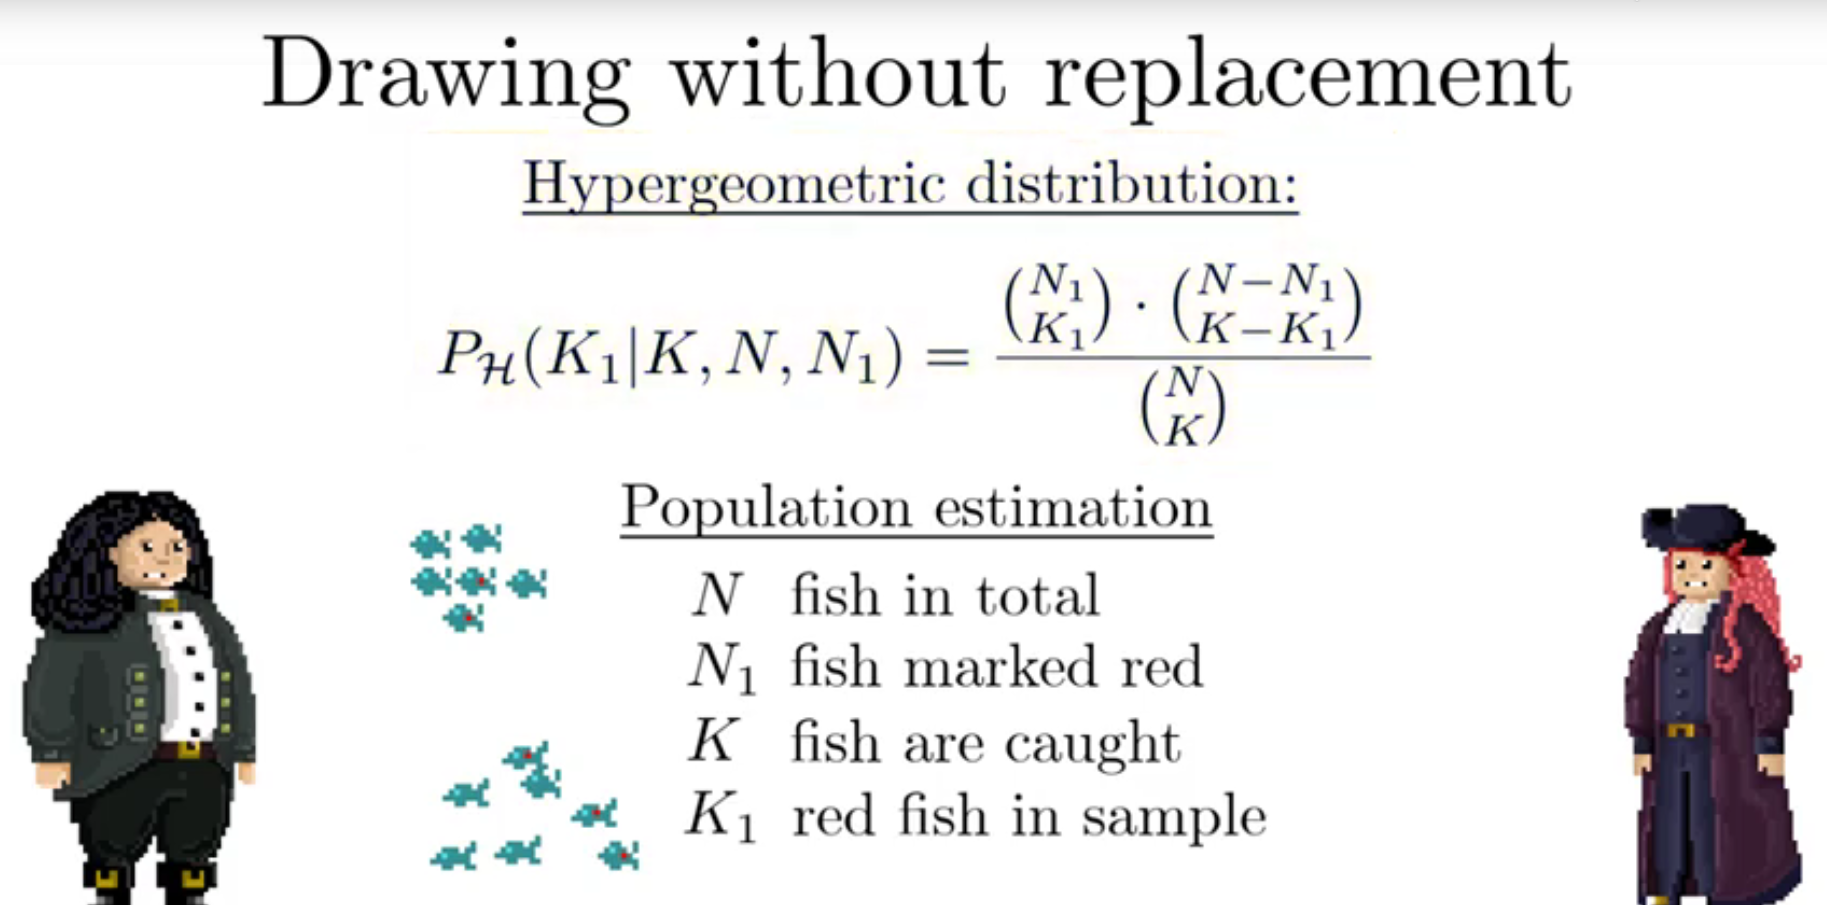
\includegraphics[width=0.75\textwidth]{4_8.png}
\end{figure}
However, in real life, the total number of fish $N$ is not known and is actually the key object of this venture.
We will learn in a future unit how Bayes’ theorem can be used to solve this inverse problem.\\

\section*{The Poisson distribution}
Now we want to consider a special limit of the binomial distribution, that will bring us to the Poisson distribution that we also saw already in the last lesson.
Consider the binomial distribution in the limit N to infinity such that the mean stays constant. Since N becomes large, Q has to go to zero and 1-Q tends to 1.
The whole expression will have non vanishing contributions only for rather small values of K, so we can approximate 1-Q by 1.
Since K is rather small compared to N we can approximate the binomial coefficient by $\frac{N^K}{K!}$
So taking this limit and forcing the mean to remain constant yields the following expression.
 \begin{figure}[H]
	\centering
	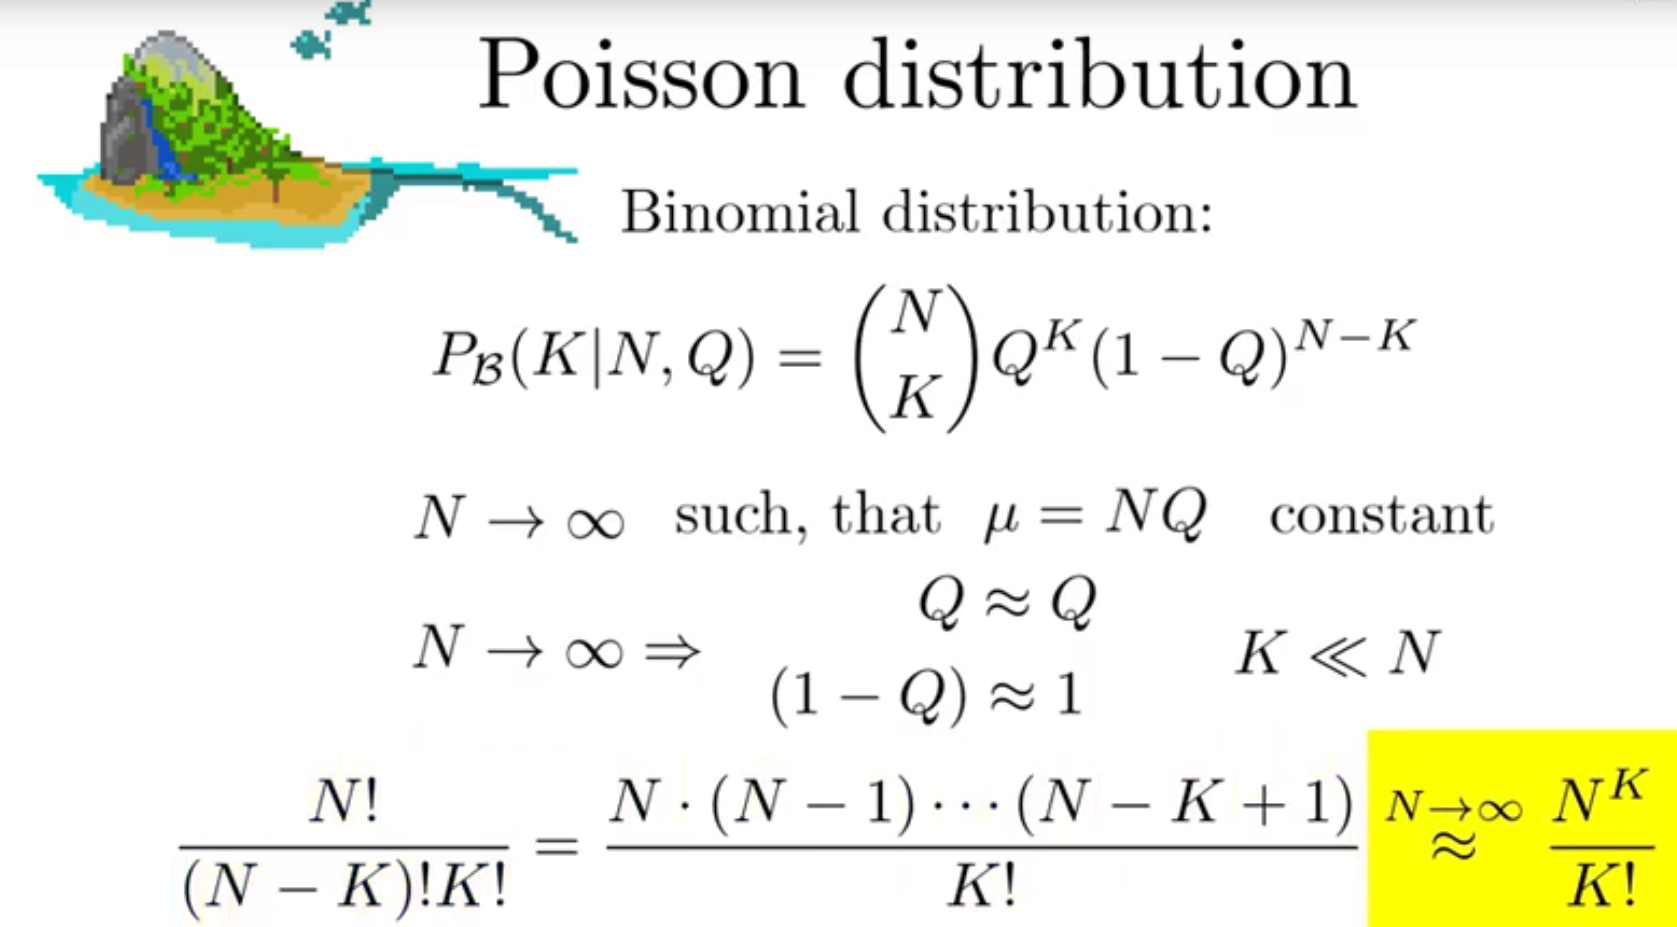
\includegraphics[width=0.75\textwidth]{4_9.png}
\end{figure}
%4_9
Along with the proper normalization we obtain the \textbf{Poisson distribution}.
%4_10
 \begin{figure}[H]
	\centering
	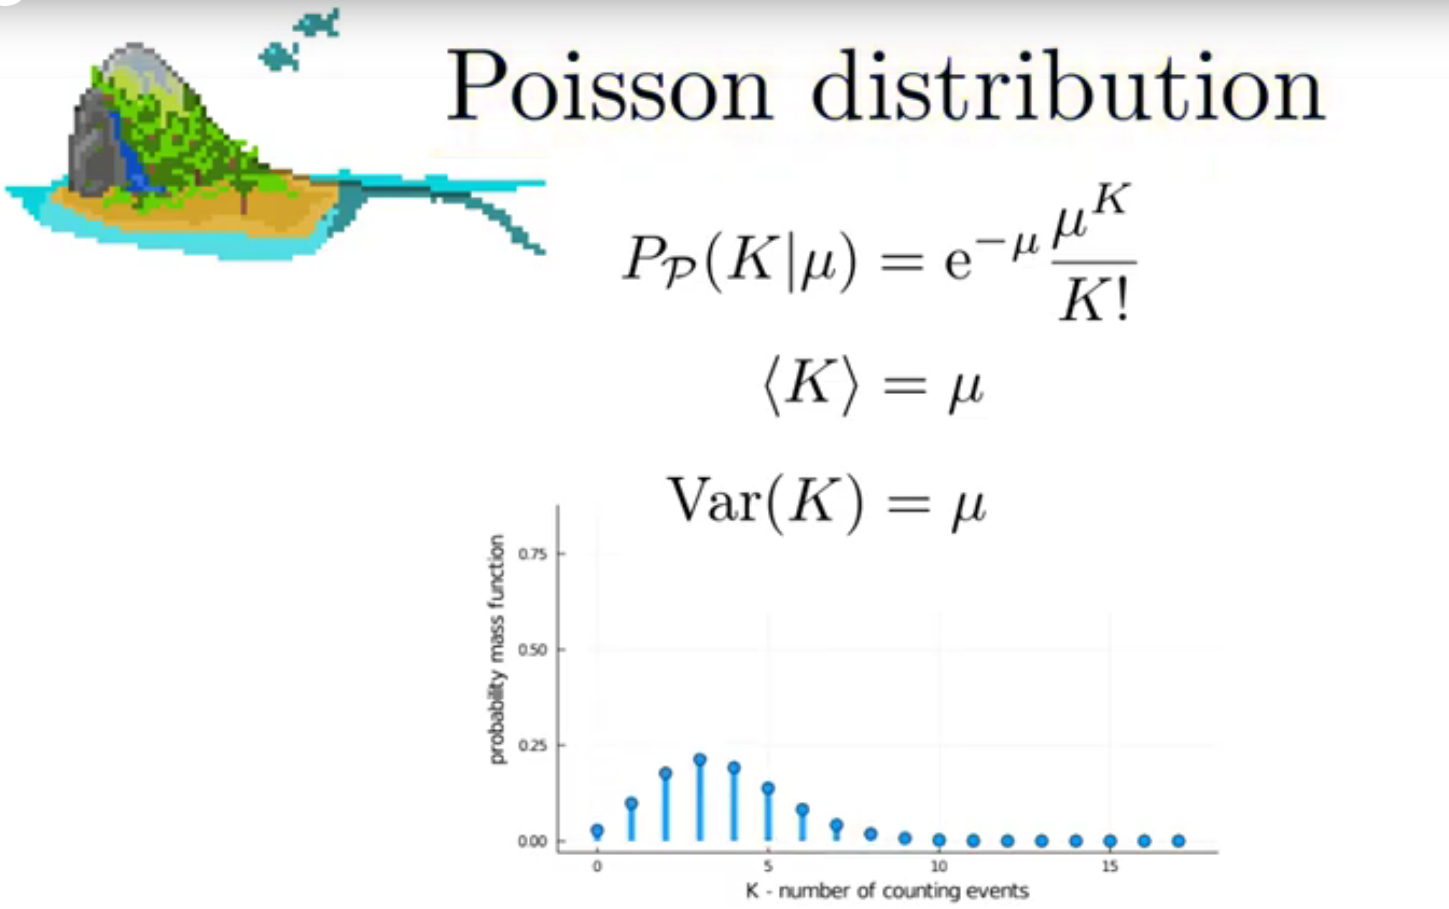
\includegraphics[width=0.75\textwidth]{4_10.png}
\end{figure}
The Poisson distribution is not only an approximation for the binomial distribution, but an important distribution with its own justification.
Assume that within an infinitesimal interval dx an event may occur or not. 
Two axioms are introduced:\\

%fbox
\fbox{\parbox{\linewidth}{
       First, the probability that an event happens within that interval dx is proportional to the length of that interval dx.\\
       Second, events in different intervals are uncorrelated.}}\\
       
Based on these axioms the probability for K events in a finite interval of length X is given by the Poisson distribution.
Poisson himself introduced this approximation for the binomial. Unfortunately he could not witness the enormous importance the distribution named after him has gained since then.\\


\section*{The geometric distribution}
Another interesting question concerns the probability that Bernoulli would have to draw K dried fruits with replacement before he gets the first apricot. The answer is the \textbf{geometric distribution}
Here Q is the probability to obtain the apricot in one draw i.e. the fraction of apricots in the pot.\\
%4_11
 \begin{figure}[H]
	\centering
	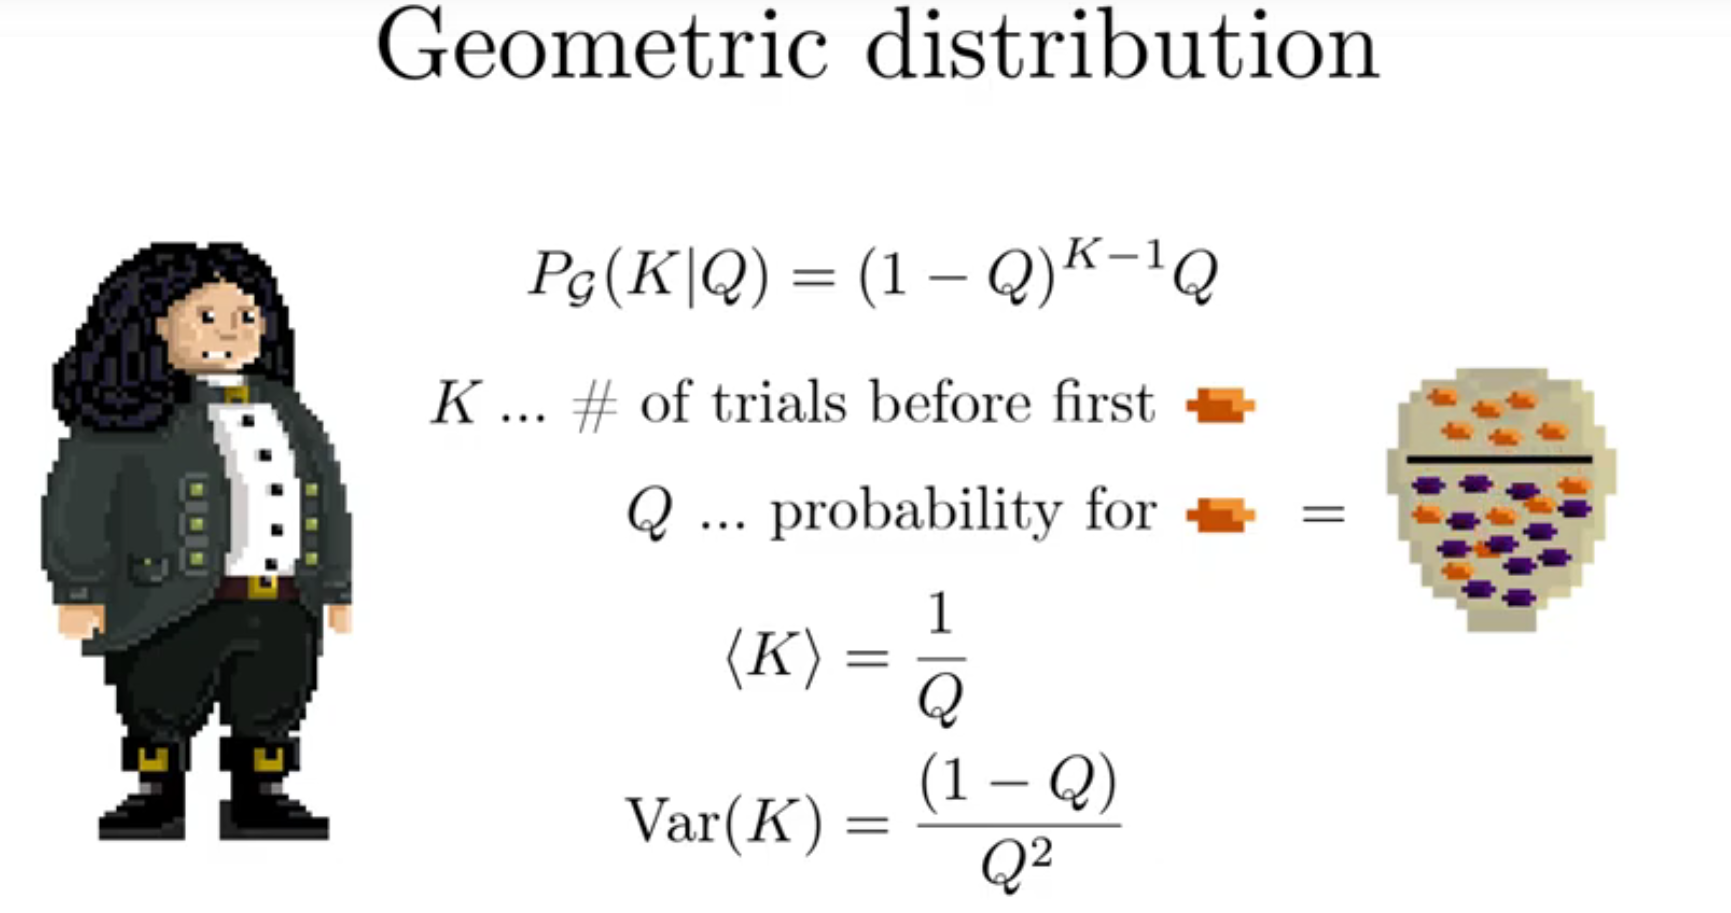
\includegraphics[width=0.75\textwidth]{4_11.png}
\end{figure}

\section{Distributing distinguishable and indistinguishable objects}
Now we turn to Laplace’s problems of distributing coins into boxes.
The coins have different features. The silver coins are \textbf{distinguishable}
and Laplace can put as many as he wants into the different boxes.
\textit{Due to the distinguishability it makes a difference to Laplace which coin goes into which box. }
Copper coins on the other hand \textbf{cannot be distinguished}. Here, only the \textit{number in a box is significant}. But this number is again arbitrary.
Gold coins are also indistinguishable but the boxes for them are such that \textit{at most one coin fits in}.\\

In the adventure, Laplace wanted to know how many ways there are to distribute N copper coins into L boxes.
The copper coins all look the same, like identical letters in a word. (It wouldn’t make any difference if you swapped two s in a word).
All that matters is the number of coins in the individual boxes. In physics such problems are called \textbf{"occupation number problems"}.\\

In other words, we ask the question how many ways there are to find L integers that add up to N. We call this a \textbf{partition} of a set of N elements into L subsets where the subsets can be empty.
A clever way to represent the possibilities graphically is to draw two red vertical lines on the x-axis. The first marks the left boundary of the first box, and the second one stands for the right boundary of the last box.
In between are L-1 blue vertical lines indicating the boundaries between adjacent boxes.
The coins in the boxes are symbolized by small circles all lined up on the x-axis.
%4_12
 \begin{figure}[H]
	\centering
	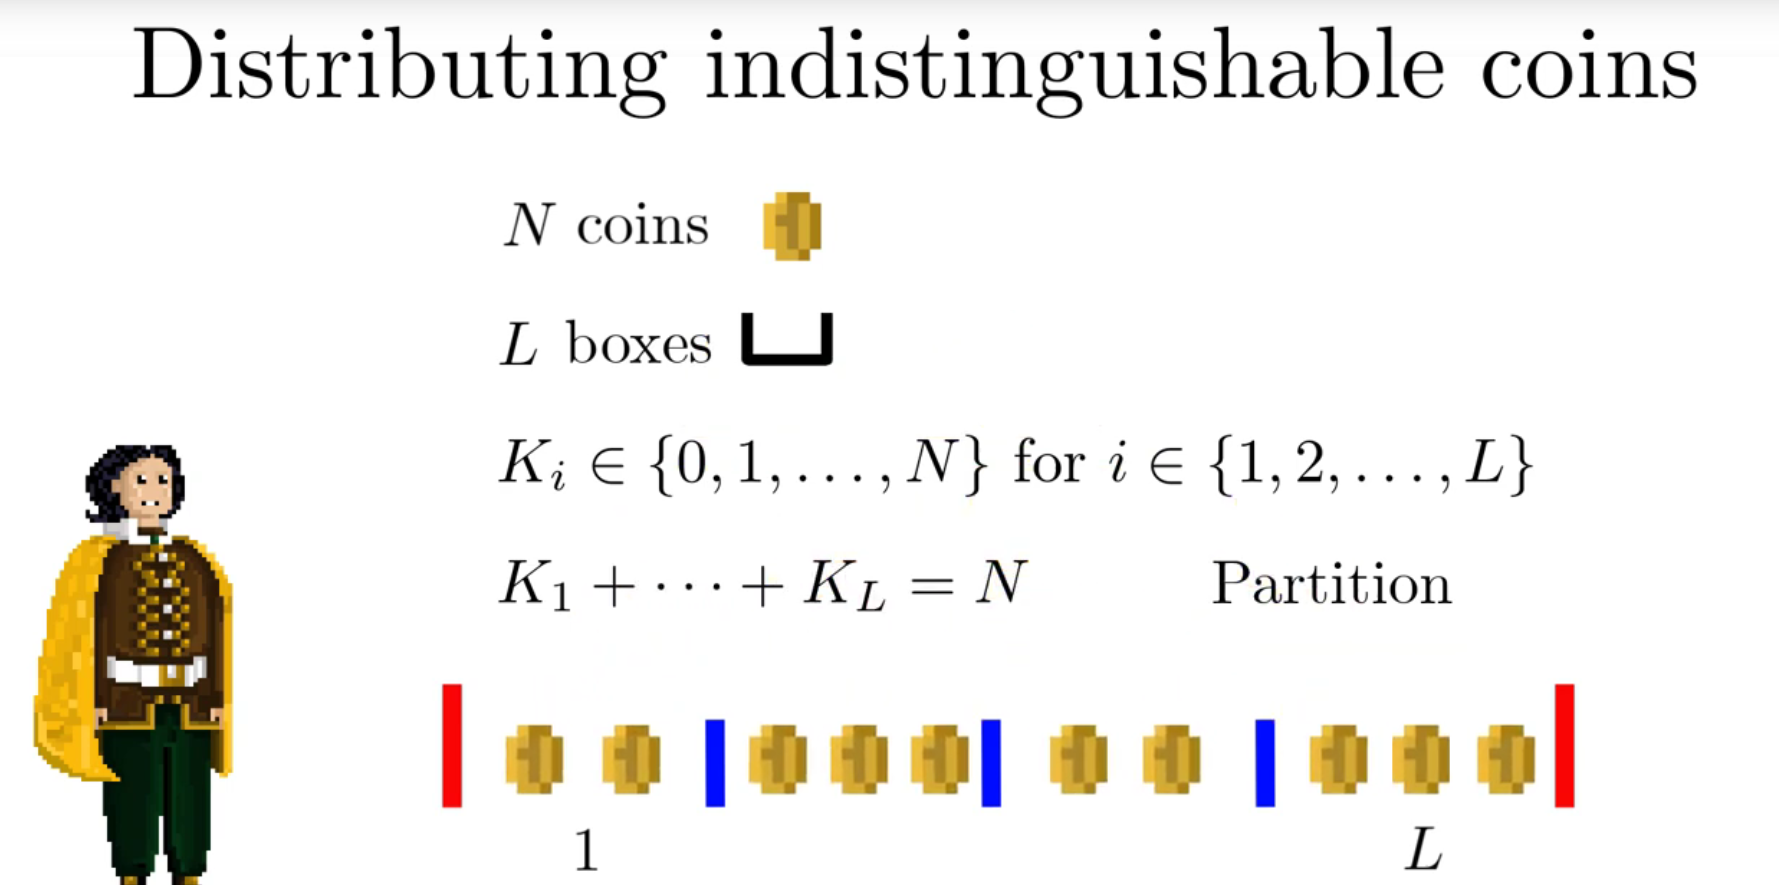
\includegraphics[width=0.75\textwidth]{4_12.png}
\end{figure}
Now it’s just like the arrangement problem with two colors we had before. There are N circles and L-1 blue lines, in total N+L-1 objects. Each combination of circles and lines on the x-axis is a valid representation of occupation numbers and vice versa. We therefore conclude the desired number of possible distributions.\\
\begin{equation*}\boxed{A_{N,L}={N+L-1\choose L-1}={N+L-1\choose N}
}\end{equation*}\\
Laplace was interested in the number of possibilities to distribute 10 copper coins into 4 boxes - the result is 286.\\
 

The situation for the gold coins is different in the sense that no more than one coin per box is allowed. In other word the \textit{occupation numbers are zero or one}. The number of ones is equal to the number of gold coins.%
 This again resembles the red-brown jar problem, with the assignment brown stands for an empty site and red for an occupied site. Hence there are 126 different arrangements.
 %4_13
 \begin{figure}[H]
	\centering
	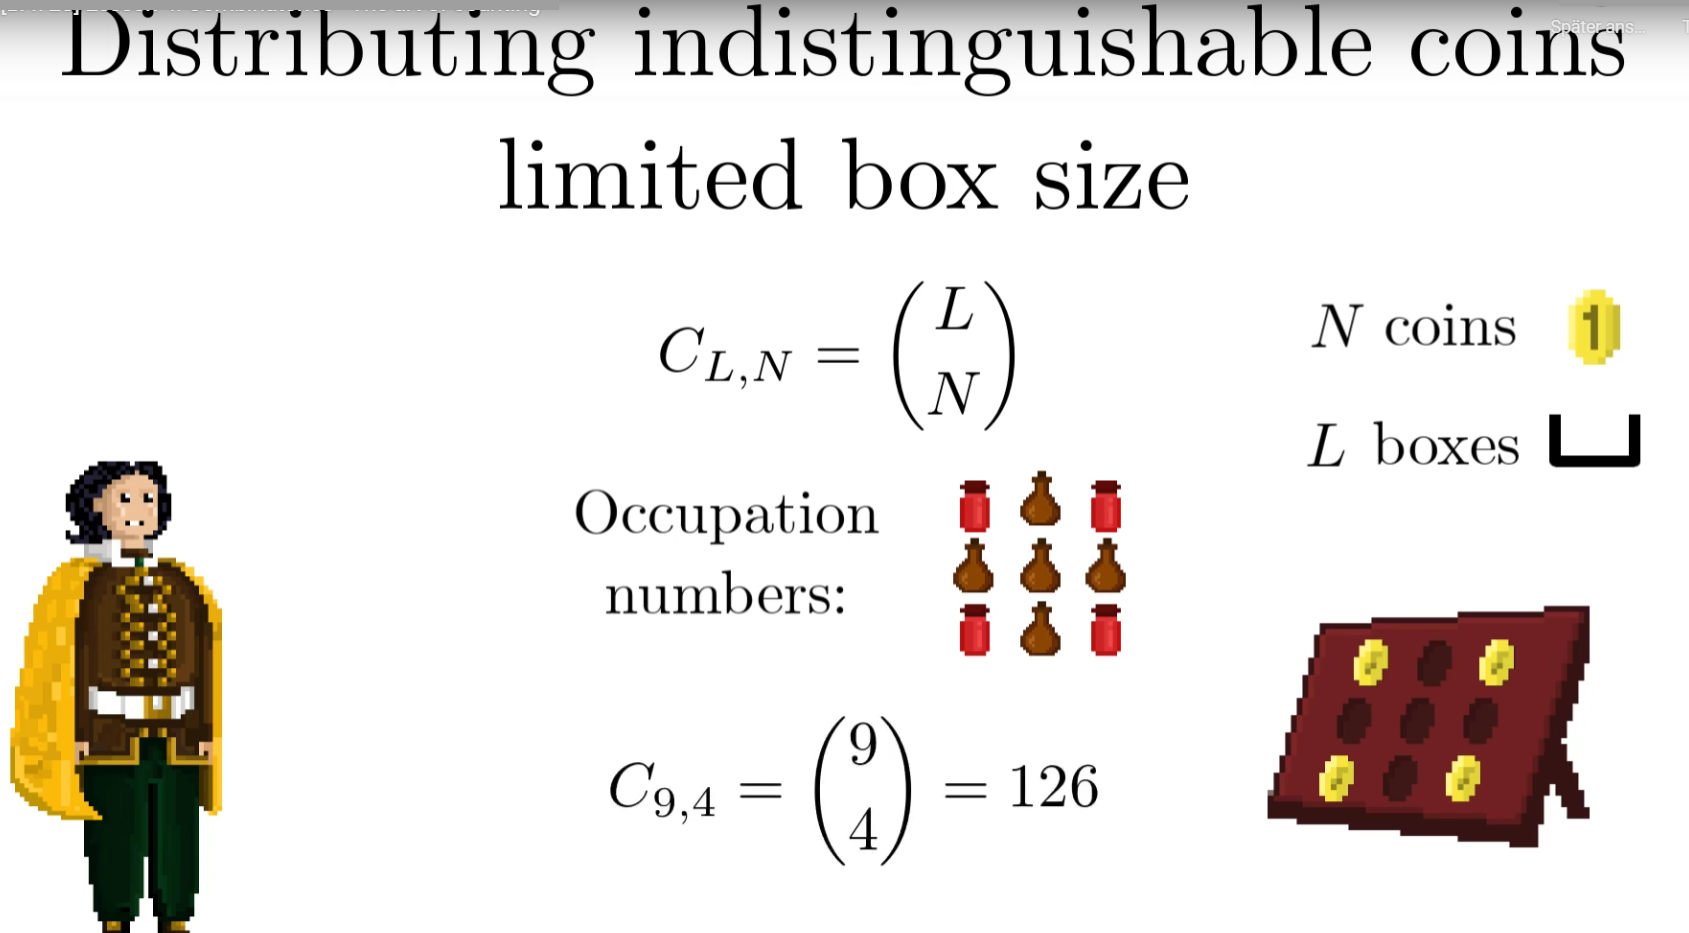
\includegraphics[width=0.75\textwidth]{4_13.png}
\end{figure}
This problem can also be viewed from a different perspective. If you enumerate the boxes from 1 to L, any valid distribution is identified by the set of box-numbers. So the problem is identical to the \textit{number of subsets of size N that can be formed}. 
As if there were L sailors who could row a boat, but Captain Bayes only needs N of them. We're looking for the different combinations to form a team. \\


Captain Bayes was pondering about the number of ways to distribute N silver coins into L boxes, where silver coins have a serial number that makes them distinguishable and the boxes are big enough to hold any number of coins.
In contrast to the copper coin problem, it now makes a difference whether a silver coin with a certain serial number, falls into box i or box j. Within a box, however, the ordering is irrelevant.\\
The problem can be split into two parts. 
First, consider a set of \textbf{occupation numbers} $K_i$ such that they add up to the total number of coins (i.e. form a partition) and determine the number of possible silver coin distributions compatible with the occupation numbers.
Second, sum over all allowed sets of occupation numbers.  \\
The first task can be related to Pascal's problem from the beginning:
Let's assume we have a valid distribution of the silver coins corresponding to the occupation numbers.
Now we erase the serial numbers and instead color the coins according to the boxes they are in. This fixes the numbers of coins with color i.
%4_14
\begin{figure}[H]
	\centering
	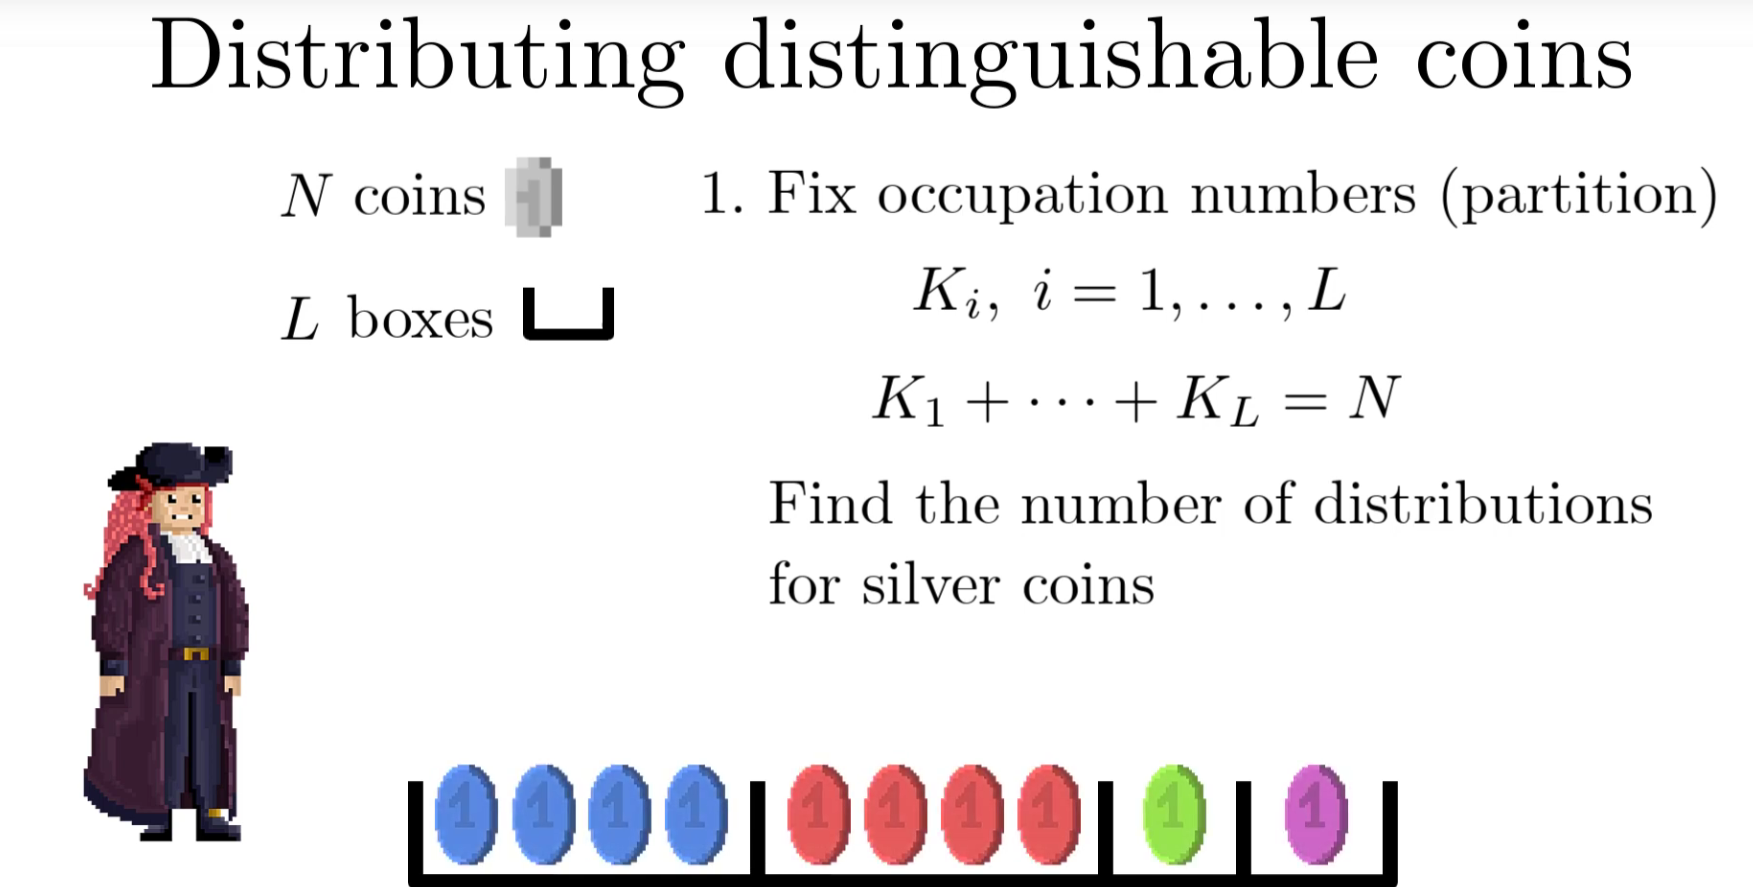
\includegraphics[width=0.75\textwidth]{4_14.png}
\end{figure}
Now we put the coins on a line and create all distinguishable color arrangements. For each one we emboss the serial number according to its position in the line and then put the coins back into the boxes according to their color. This procedure generates all desired distributions of silver coins.%%
The number of possibilities is given by the multinomial coefficient.\\

The second step is to \textit{sum the multinomial coefficients over all sets of admissible occupancy numbers}. 
\begin{equation*}\boxed{\sum_{\{K_i\},\sum_iK_i=N}{N\choose\{K_i\}}
}\end{equation*}\\
There are N+K-1 choose N such sets, but there is a trick to evaluate this sum:\\
Identifying the multinomial theorem leads to the the simple result: 
\begin{equation*}\boxed{(1+1+...+1)^N=\sum_{\{K_i\},\sum_iK_i=N}{N\choose\{K_i\}}1^N=L^N
}\end{equation*}\\

This is the same as the number of ordered samples of size N from a population of size L with replacement, like forming words from an alphabet.
In the adventure the task was to distribute 10 silver coins into 4 boxes. Thanks to the trick, we don't have to evaluate and sum over the 286 multinomial coefficients but instead obtain directly the result 4 to the power of 10, resulting approximately in one million possible configurations.
That is equal to the number of 10-character-words using only four letters, 
or the number of gene sequences with ten base pairs.\\


This concludes the forth unit. Deepen your understanding of combinatorics by looking at different examples and experimenting with the interactive simulations, feel free to ask questions in the forum and feel encouraged to test your knowledge in the quiz!



\end{document}